\documentclass[aspectratio=169]{beamer}

\usepackage{xcolor}
\usepackage{lmodern}
\usepackage[normalem]{ulem}
\usepackage{tcolorbox}
\usepackage{graphicx}

\definecolor{IllinoisOrange}{RGB}{232,74,39}
\definecolor{IllinoisBlue}{RGB}{19,41,75}

\usetheme{default}
\usefonttheme[onlymath]{serif}                    % use serif math
\setbeamercolor{structure}{fg=IllinoisOrange}     % set main text color
\setbeamercolor{normal text}{fg=IllinoisBlue}     % set main text color
\setbeamertemplate{headline}{}                    % modify the headline to be null
\setbeamercolor{frametitle}{bg=}                  % set frametitle background
\setbeamercolor{frametitle}{fg=IllinoisOrange}    % set the frametitle foreground
\setbeamersize{text margin left=0.15in,
               text margin right=0.15in}          % set the text margins
\setbeamertemplate{navigation symbols}{}          % turn off navigation line
\setbeamertemplate{enumerate items}[default]      % turn off the balls for enumerate
\setbeamertemplate{itemize subitem}{$\bullet$}    % set subitem bullets
\setbeamertemplate{itemize subsubitem}{$*$}       % set subsubitem bullets
\setbeamercolor{alerted text}{fg=IllinoisOrange}  % color alert text

% Modify the footline to only have the page numbering in the center, nothing else
\makeatletter
\setbeamertemplate{footline}
{
 \leavevmode%
 \hbox{\begin{beamercolorbox}[wd=\paperwidth,ht=2.25ex,dp=1ex]{}%
     \usebeamerfont{author in head/foot}%
     \hspace*{0.02in}
     \raisebox{-0.0in}{
\includegraphics[height=0.21in]{./media/UILogoBlockI.pdf}}%
     \hfill\hspace*{0.8in}\insertframenumber{}
     \hfill\raisebox{-0.07in}{
\includegraphics[height=0.3in]{./media/ceesd-logo-2.pdf}}%
 \end{beamercolorbox}}
 \vskip0pt%
}

% Set frame title to properly center the text
\setbeamertemplate{frametitle}
{
  \leavevmode%
  \hbox{%
  \begin{beamercolorbox}[wd=\paperwidth,ht=2.5ex,dp=0ex]{frametitle}%
    \raggedright
    \bfseries
    \hspace*{0.3em}%
    \usebeamerfont{frametitle}\insertframetitle
  \end{beamercolorbox}}
  \vspace*{-2.75ex}
}

\makeatother

\begin{document}

\begin{frame}\frametitle{}

  \vspace*{0.2in}

  \hspace*{0.0in}\textrm{{\huge\bfseries\color{IllinoisOrange} NUWEST: NNSA-University Workshop on Exascale Simulation Technologies}}

  \vspace*{0.2in}
  \hrule
  \begin{center}
    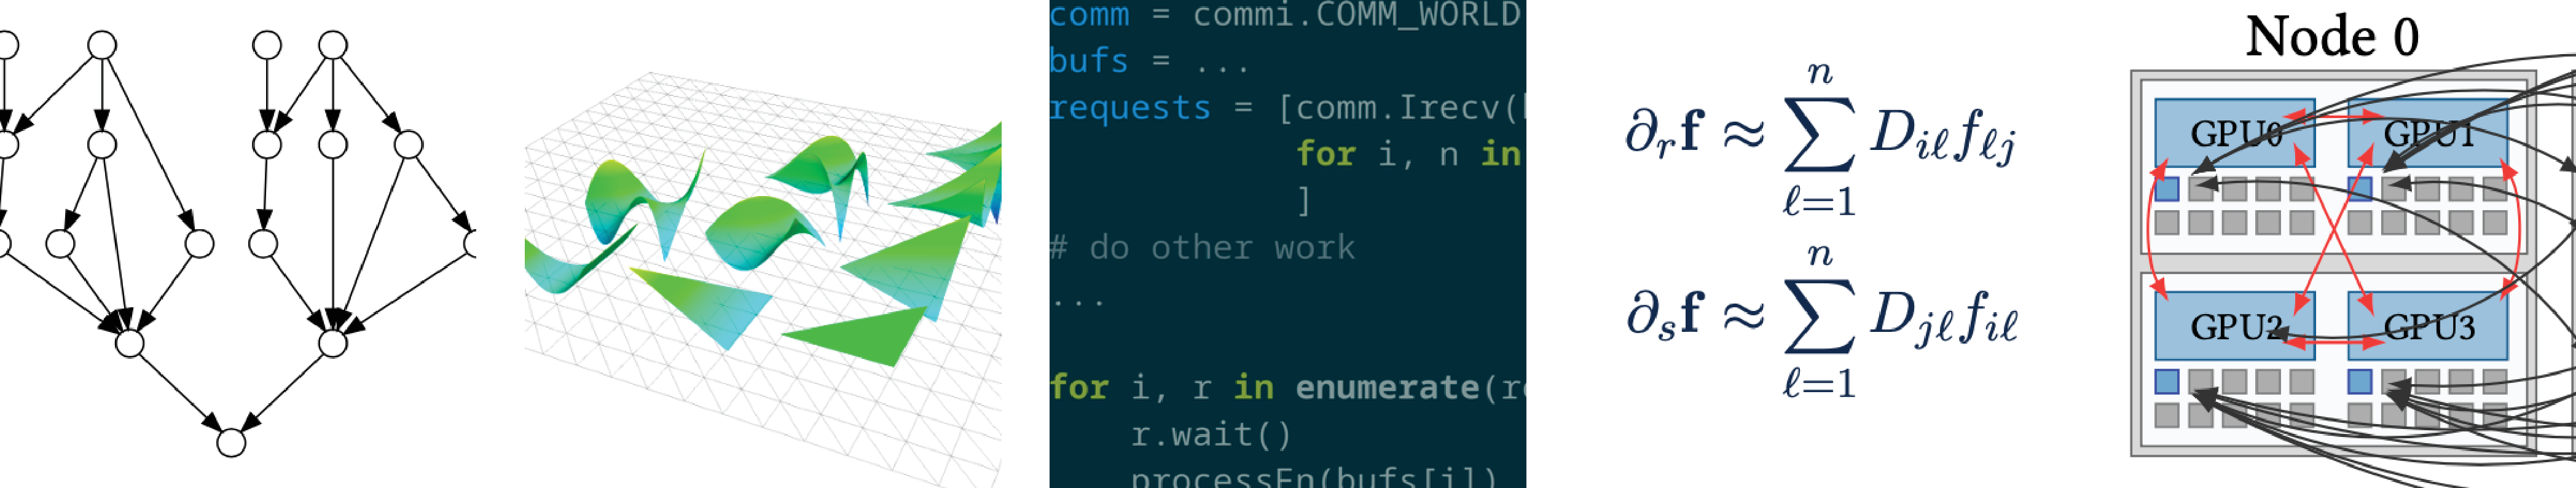
\includegraphics[width=0.75\textwidth]{./media/coverart-cs.pdf}
  \end{center}
  \hrule

  \vspace*{0.1in}
  \noindent\textit{January 18, 2024}\\
  \vspace*{0.1in}
  \noindent\textbf{\color{IllinoisOrange}Luke Olson}\\
  \noindent{\color{IllinoisOrange}University of Illinois Urbana-Champaign}\\

\end{frame}

\begin{frame}{NUWEST's Goal}
  \begin{center}
    \begin{tcolorbox}[colframe=IllinoisOrange]
      To share ideas on tools for exascale predictive science
    \end{tcolorbox}
  \end{center}
  \begin{itemize}
    \item Showcase and characterize available technologies
    \item Identify challenges and limitations
    \item Provide opportunities to initiate collaboration
    \item Focus on \alert{hands-on experience}~---~technologies to look at in detail
  \end{itemize}
\end{frame}

\begin{frame}{Schedule}
  \begin{tcolorbox}[colframe=IllinoisOrange]
    https://illinois-ceesd.github.io/nuwest/
  \end{tcolorbox}
  \begin{itemize}
    \item \alert{Keynote 1} [Christian Trott, Sandia]
    \item \alert{Keynote 2} [Bill Gropp, Illinois]
    \item \alert{Conceptual Overview} (4\texttimes{} 10--12 min, morning/afternoon) \alert{Ballroom}
    \item Small group interactions: \alert{hands-on} (2h window) \alert{In parallel}\\
      \only<1>{
        \medskip
        \alert{Morning}:
        \begin{itemize}
          \item Scalable and portable HPC in Python using Parla and PyKokkos {\tiny\color{gray}George Biros, University of Texas at Austin}
          \item Parsl - Python based workflow management {\tiny\color{gray}Daniel S. Katz, Doug Friedel, University of Illinois Urbana-Champaign}
          \item Pragmatic performance-portable solids and fluids\\ with Ratel, libCEED, and PETSc {\tiny\color{gray}Jed Brown, University of Colorado Boulder}
          \item CUnumeric and Legion {\tiny\color{gray}Charlelie Laurent, Stanford University}
        \end{itemize}
      }
      \only<2>{
        \medskip
        \alert{Afternoon}:
        \begin{itemize}
          \item OpenCilk: A Modular and Extensible Software Infrastructure\\ for Fast Task-Parallel Code {\tiny\color{gray} Tao Schardl, Massachusetts Institute of Technology }
          \item MIRGE -- A lazy evaluation framework in Python {\tiny\color{gray} Andreas Kloeckner, University of Illinois Urbana-Champaign }
          \item MPI Advance - Optimizations and Extensions to MPI {\tiny\color{gray} Purushotham V. Bangalore, University of Alabama }
          \item Acceleration and Abstraction of Python based Monte Carlo Compute Kernels for Heterogeneous machines via Numba {\tiny\color{gray} Joanna Piper Morgan, Oregon State University }
        \end{itemize}
      }
    \item View as 1 hour + 1 hour: try another session at the 1 hour mark!
  \end{itemize}
\end{frame}

\begin{frame}{Logistics}
  \begin{itemize}
    \item \url{https://illinois-ceesd.github.io/nuwest}
    \item Contact Luke Olson (\texttt{lukeo@illinois.edu}) or\\
      \hspace{1.25cm} Courtney McLearin (\texttt{cmcleari@illinois.edu}).
    \item See Slack for announcements
    \item {\color{IllinoisOrange} \texttt{0800-0900}} Keynotes
    \item {\color{IllinoisOrange} \texttt{0900-1200}} Morning session
    \item {\color{IllinoisOrange} \texttt{1200-1300}} Lunch (on site)
    \item {\color{IllinoisOrange} \texttt{1300-1600}} Afternoon session
    \item {\color{IllinoisOrange} \texttt{1600-1700}} Closing + collaboration time
    \item {\color{IllinoisOrange} \texttt{1700-1900}} Optional social @ Bow \& Arrow Brewing Co.
  \end{itemize}
\end{frame}

\begin{frame}{Some questions to think about:}
  \begin{itemize}
    \item What ideas are working for \uline{actual} \uline{simulations}?
    \item Any pivots needed?
    \item What are lab needs?
    \item What are barriers for adoption on conceivable hardware?
    \item How do tools improve with end-to-end simulation workflows?
  \end{itemize}
\end{frame}

\begin{frame}\frametitle{}
  \vspace*{0.2in}
  \begin{center}
    \vspace*{0.35in}

    \textbf{\huge\color{IllinoisOrange} Questions?}

    \vspace*{0.5in}
    This material is based in part upon work supported by the Department of Energy,
    National Nuclear Security Administration, under Award Number DE-NA0003963. 
  \end{center}
\end{frame}

\begin{frame}{Feedback:}
  \begin{tcolorbox}[colframe=IllinoisOrange]
    \url{TODO}
  \end{tcolorbox}
  \begin{itemize}
    \item In the context of real, predictive simulation, for the technologies
      you observed list one or two pivots needed for adoption.  i.e., what
      would it take to effectively use technology XYZ?
    \item List any barriers for adoption on conceivable hardware.
    \item List one or two lab needs not necessary covered or addressed by the
      suite of presented technologies.
    \item How do you foresee  end-to-end simulation workflows impacting
      exacscale technologies?  List one or two observations.
  \end{itemize}
\end{frame}

\end{document}
